% 2026-10-22：横轴显示名称采用表1缩写并保留比特数；仅改xticklabels，不改内部线路标识与168个数据值。
% 2026-10-22作者指示：本图改回单栏，按栏宽居中，保留全部原数据。
% cxy批注修改：保真度图通栏排版，坐标及图例使用small字号，保留全部线路及原数据。
% Compile manuscript_english.tex.
\begin{figure}[!htbp]\centering

\par\begingroup\centering\begin{minipage}{\linewidth}\centering
{\resizebox{\linewidth}{!}{%
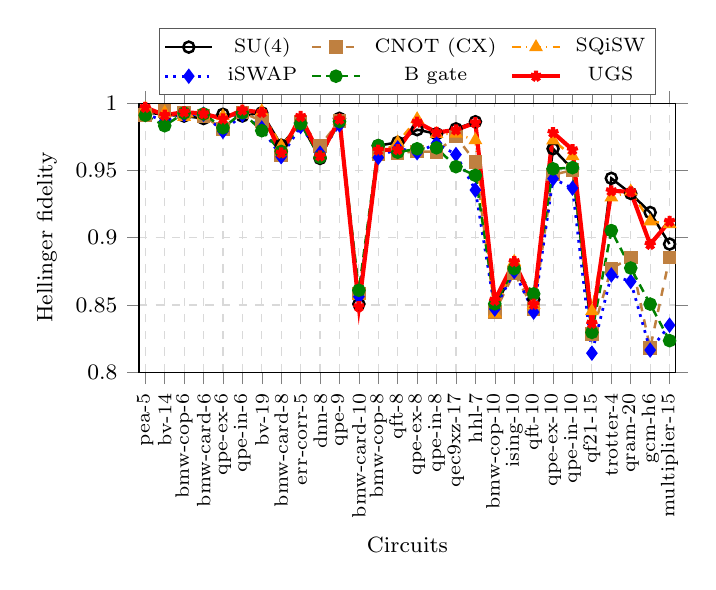
\begin{tikzpicture}
\begin{axis}[
    width=8.4cm,
    height=5.0cm,
    xlabel={Circuits},
    ylabel={Hellinger fidelity},
    symbolic x coords={{pea\_n5},{bv\_n14},{bmw\_quark\_copula\_n6},{bmw\_quark\_cardinality\_n6},{qpeexact\_n6},{qpeinexact\_n6},{bv\_n19},{bmw\_quark\_cardinality\_n8},{error\_correctiond3\_n5},{dnn\_n8},{qpe\_n9},{bmw\_quark\_cardinality\_n10},{bmw\_quark\_copula\_n8},{qft\_8},{qpeexact\_n8},{qpeinexact\_n8},{qec9xz\_n17},{hhl\_n7},{bmw\_quark\_copula\_n10},{ising\_n10},{qft\_10},{qpeexact\_n10},{qpeinexact\_n10},{qf21\_n15},{basis\_trotter\_n4},{qram\_n20},{gcm\_h6},{multiplier\_n15}},
    xtick=data,
    xticklabels={pea-5,bv-14,bmw-cop-6,bmw-card-6,qpe-ex-6,qpe-in-6,bv-19,bmw-card-8,err-corr-5,dnn-8,qpe-9,bmw-card-10,bmw-cop-8,qft-8,qpe-ex-8,qpe-in-8,qec9xz-17,hhl-7,bmw-cop-10,ising-10,qft-10,qpe-ex-10,qpe-in-10,qf21-15,trotter-4,qram-20,gcm-h6,multiplier-15},
    x tick label style={rotate=90,anchor=east,font=\scriptsize},
    y tick label style={font=\footnotesize},
    label style={font=\footnotesize},
    ymin=0.80,
    ymax=1.00,
    ytick={0.80,0.85,0.90,0.95,1.00},
    grid=major,
    grid style={dashed,gray!30},
    tick align=outside,
    enlarge x limits=0.012,
    legend style={
        at={(0.5,1.03)},
        anchor=south,
        legend columns=3,
        draw=black!65,
        fill=white,
        line width=.3pt,
        inner sep=1.5pt,
        row sep=0pt,
        /tikz/column sep=3pt,
        font=\scriptsize
    },
    clip=true,
]
\addplot+[black, solid, mark=o, mark options={solid}, line width=0.9pt] coordinates {({pea\_n5},0.993164) ({bv\_n14},0.991388) ({bmw\_quark\_copula\_n6},0.990376) ({bmw\_quark\_cardinality\_n6},0.988548) ({qpeexact\_n6},0.991699) ({qpeinexact\_n6},0.990402) ({bv\_n19},0.992805) ({bmw\_quark\_cardinality\_n8},0.968719) ({error\_correctiond3\_n5},0.985368) ({dnn\_n8},0.958884) ({qpe\_n9},0.988668) ({bmw\_quark\_cardinality\_n10},0.850709) ({bmw\_quark\_copula\_n8},0.968371) ({qft\_8},0.970843) ({qpeexact\_n8},0.980225) ({qpeinexact\_n8},0.977166) ({qec9xz\_n17},0.980858) ({hhl\_n7},0.986127) ({bmw\_quark\_copula\_n10},0.848517) ({ising\_n10},0.876546) ({qft\_10},0.854017) ({qpeexact\_n10},0.966064) ({qpeinexact\_n10},0.950906) ({qf21\_n15},0.828439) ({basis\_trotter\_n4},0.944092) ({qram\_n20},0.932861) ({gcm\_h6},0.918714) ({multiplier\_n15},0.895264)};
\addlegendentry{SU(4)}
\addplot+[brown, dashed, mark=square*, mark options={solid}, line width=0.9pt] coordinates {({pea\_n5},0.991211) ({bv\_n14},0.994185) ({bmw\_quark\_copula\_n6},0.993098) ({bmw\_quark\_cardinality\_n6},0.990447) ({qpeexact\_n6},0.980713) ({qpeinexact\_n6},0.992880) ({bv\_n19},0.986839) ({bmw\_quark\_cardinality\_n8},0.961020) ({error\_correctiond3\_n5},0.986186) ({dnn\_n8},0.968193) ({qpe\_n9},0.986726) ({bmw\_quark\_cardinality\_n10},0.858434) ({bmw\_quark\_copula\_n8},0.962214) ({qft\_8},0.962917) ({qpeexact\_n8},0.964111) ({qpeinexact\_n8},0.963735) ({qec9xz\_n17},0.975274) ({hhl\_n7},0.956247) ({bmw\_quark\_copula\_n10},0.844809) ({ising\_n10},0.873838) ({qft\_10},0.846908) ({qpeexact\_n10},0.946777) ({qpeinexact\_n10},0.950150) ({qf21\_n15},0.828277) ({basis\_trotter\_n4},0.876953) ({qram\_n20},0.885254) ({gcm\_h6},0.817903) ({multiplier\_n15},0.885254)};
\addlegendentry{CNOT (CX)}
\addplot+[orange!85!yellow, dashdotted, mark=triangle*, mark options={solid}, line width=0.9pt] coordinates {({pea\_n5},0.995850) ({bv\_n14},0.992940) ({bmw\_quark\_copula\_n6},0.989777) ({bmw\_quark\_cardinality\_n6},0.990835) ({qpeexact\_n6},0.990234) ({qpeinexact\_n6},0.993466) ({bv\_n19},0.993880) ({bmw\_quark\_cardinality\_n8},0.968106) ({error\_correctiond3\_n5},0.985079) ({dnn\_n8},0.961826) ({qpe\_n9},0.986829) ({bmw\_quark\_cardinality\_n10},0.857001) ({bmw\_quark\_copula\_n8},0.962008) ({qft\_8},0.970701) ({qpeexact\_n8},0.988088) ({qpeinexact\_n8},0.977069) ({qec9xz\_n17},0.977322) ({hhl\_n7},0.972472) ({bmw\_quark\_copula\_n10},0.843636) ({ising\_n10},0.882038) ({qft\_10},0.850084) ({qpeexact\_n10},0.972275) ({qpeinexact\_n10},0.960685) ({qf21\_n15},0.845339) ({basis\_trotter\_n4},0.929932) ({qram\_n20},0.934326) ({gcm\_h6},0.912179) ({multiplier\_n15},0.910156)};
\addlegendentry{SQiSW}
\addplot+[blue, dotted, mark=diamond*, mark options={solid}, line width=1.0pt] coordinates {({pea\_n5},0.991943) ({bv\_n14},0.986686) ({bmw\_quark\_copula\_n6},0.991502) ({bmw\_quark\_cardinality\_n6},0.991728) ({qpeexact\_n6},0.979004) ({qpeinexact\_n6},0.991205) ({bv\_n19},0.981444) ({bmw\_quark\_cardinality\_n8},0.960165) ({error\_correctiond3\_n5},0.982641) ({dnn\_n8},0.962829) ({qpe\_n9},0.983833) ({bmw\_quark\_cardinality\_n10},0.856065) ({bmw\_quark\_copula\_n8},0.959589) ({qft\_8},0.966602) ({qpeexact\_n8},0.963135) ({qpeinexact\_n8},0.970093) ({qec9xz\_n17},0.961741) ({hhl\_n7},0.935372) ({bmw\_quark\_copula\_n10},0.847001) ({ising\_n10},0.874839) ({qft\_10},0.844711) ({qpeexact\_n10},0.943848) ({qpeinexact\_n10},0.936805) ({qf21\_n15},0.814201) ({basis\_trotter\_n4},0.872314) ({qram\_n20},0.867432) ({gcm\_h6},0.816479) ({multiplier\_n15},0.834961)};
\addlegendentry{iSWAP}
\addplot+[green!50!black, densely dashed, mark=otimes*, mark options={solid}, line width=0.9pt] coordinates {({pea\_n5},0.990967) ({bv\_n14},0.983186) ({bmw\_quark\_copula\_n6},0.992640) ({bmw\_quark\_cardinality\_n6},0.991973) ({qpeexact\_n6},0.981689) ({qpeinexact\_n6},0.992834) ({bv\_n19},0.979489) ({bmw\_quark\_cardinality\_n8},0.964063) ({error\_correctiond3\_n5},0.984672) ({dnn\_n8},0.959726) ({qpe\_n9},0.986265) ({bmw\_quark\_cardinality\_n10},0.860904) ({bmw\_quark\_copula\_n8},0.968432) ({qft\_8},0.963470) ({qpeexact\_n8},0.966064) ({qpeinexact\_n8},0.966731) ({qec9xz\_n17},0.952747) ({hhl\_n7},0.946303) ({bmw\_quark\_copula\_n10},0.850806) ({ising\_n10},0.876972) ({qft\_10},0.858218) ({qpeexact\_n10},0.951172) ({qpeinexact\_n10},0.952027) ({qf21\_n15},0.829598) ({basis\_trotter\_n4},0.905273) ({qram\_n20},0.877441) ({gcm\_h6},0.850649) ({multiplier\_n15},0.823486)};
\addlegendentry{B gate}
\addplot+[red, solid, mark=star, mark options={solid}, line width=1.5pt] coordinates {({pea\_n5},0.996826) ({bv\_n14},0.990959) ({bmw\_quark\_copula\_n6},0.993354) ({bmw\_quark\_cardinality\_n6},0.992141) ({qpeexact\_n6},0.988281) ({qpeinexact\_n6},0.994800) ({bv\_n19},0.993051) ({bmw\_quark\_cardinality\_n8},0.962918) ({error\_correctiond3\_n5},0.990013) ({dnn\_n8},0.960744) ({qpe\_n9},0.988034) ({bmw\_quark\_cardinality\_n10},0.848750) ({bmw\_quark\_copula\_n8},0.965035) ({qft\_8},0.965458) ({qpeexact\_n8},0.985752) ({qpeinexact\_n8},0.978153) ({qec9xz\_n17},0.980089) ({hhl\_n7},0.985365) ({bmw\_quark\_copula\_n10},0.853500) ({ising\_n10},0.882169) ({qft\_10},0.850534) ({qpeexact\_n10},0.978114) ({qpeinexact\_n10},0.965304) ({qf21\_n15},0.836409) ({basis\_trotter\_n4},0.934814) ({qram\_n20},0.934082) ({gcm\_h6},0.895036) ({multiplier\_n15},0.912109)};
\addlegendentry{UGS}
\end{axis}
\end{tikzpicture}
}}
\par\end{minipage}\par\endgroup

\vspace{2pt}
\caption{Fidelity comparison across 28 circuits under a fully connected topology.}\label{fig:11}
% 翻译：图11：全连接拓扑下的线路保真度比较。
\end{figure}
